\chapter{Introduction}
Cryptocurrencies provide us with a mechanism to send a unit of cryptocurrency to anyone, directly, anywhere. Cryptocurrencies are entirely virtual; there are no physical coins, or even digital coins per se. There are no banks involved, no mediators and no central reserve controlling coin supply; what cryptocurrencies often have, however, are cryptography principles such as elliptic curve cryptography and one-way hash functions that help secure ownership of funds. Cryptocurrencies can be classified by their ability to establish ownership, protecting against double spending, ensuring anonymity/privacy and minting new currency \cite{RefWorks:doc:5cfe1c72e4b096a2b4747aac}. 
\\\\
There are several leading cryptocurrencies which, together, dominate the cryptocurrency market capitalisation [see figure \ref{fig:cryptocurrency-capitalisaiton}]. The biggest player of all leading cryptocurrencies is Bitcoin. 

\begin{figure}[h!]
  \centering
  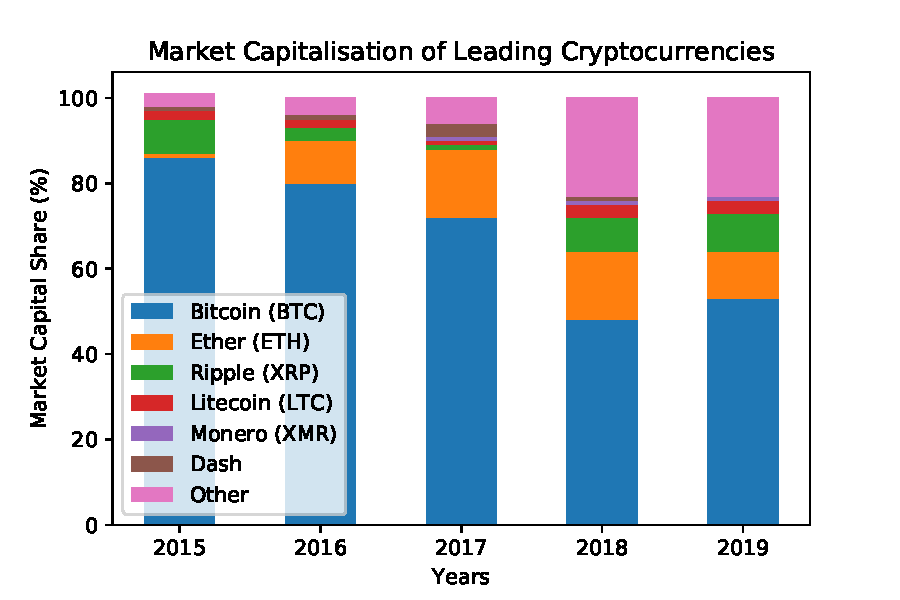
\includegraphics[width = 12cm]{./figures/marketcapitalisation.pdf}\\[0.5cm] 
  \caption{Market Capitalisation of leading Cryptocurrencies from 2015-2019  \cite{RefWorks:doc:5cfe03c0e4b091a4a00f7e76}}
  \label{fig:cryptocurrency-capitalisaiton}
\end{figure}


\section{Bitcoin}
Bitcoin is a cryptocurrency that has become a household name in recent years, it dominated news headlines on several occasions in 2017 as its price dramatically climbed and peaked at over \$19,000 in December 2017, a 1,824\% value increase since January of the same year \cite{RefWorks:doc:5cfb6adce4b03a90bd6e557d}. What may not be as widely known is the excellent vehicle and tool Bitcoin can be for illegal activity. Bitcoin's relative lack of tractability, perceived anonymity and lack of regulatory oversight \cite{RefWorks:doc:5cfb837fe4b0d23f20773924}, compared to traditional fiat currencies, has rapidly attracted criminals such as illegal arms dealers, kidnappers, people smugglers, drug traffickers, blackmailers and terrorism financers \cite{RefWorks:doc:5cfb79e2e4b0132e0223fff6} \cite{RefWorks:doc:5c49e7c4e4b0d339f6625a91}.
\\\\
This unregulated nature of cryptocurrencies has been a cause of great concern for governing bodies; the Chinese government banned residents from trading cryptocurrencies in 2017 and the Bank of England's Governer Mark Carney has publicly expressed concerns about cryptocurrencies \cite{RefWorks:doc:5cfbc8fee4b05850fa02e710}. 
Recent studies have estimated over a quarter of all Bitcoin users (26\%) and nearly half of all Bitcoin transactions (46\%) are associated with illegal activity \cite{RefWorks:doc:5cfbc8fee4b05850fa02e710}; in March 2017 46\% of Bitcoin's transaction value equated to \$76 billion, which is close to the scale of the US and European markets for illegal drugs \cite{RefWorks:doc:5cfbc8fee4b05850fa02e710}. Despite numerous 'darknet' marketplace seizures, such as the infamous Silk Road which was shut down by the FBI in 2014 who seized over \$4 million worth of bitcoin \cite{RefWorks:doc:5cfbc8fee4b05850fa02e710}, the amount of illegal activity associated with bitcoin remained close to it's all time high as of April 2017 \cite{RefWorks:doc:5cfbc8fee4b05850fa02e710}. 
\\\\
However, many cryptocurrencies have a distinct weakness for those wishing to evade the law; every transaction is published on the 'public ledger' that is the Blockchain and will remain forever accessible. Meanwhile, the capability of digital forensic tools advance further as research into de-anonymising Bitcoin activity continues. Right now, the individual identities of users may be masked by the pseudo-anonymity of their Bitcoin address, but through heuristics based on idioms of use, knowledge of wallet software and even analysis of user behaviour, Bitcoin addresses can be grouped into \textit{clusters} [see \ref{background:clustering}] of addresses known to be controlled by a single user. Combine such clustering with a graphical, interactive representation of Blockchain data and suddenly Bitcoin activity becomes more transparent and digital forensic investigations are made more accessible. 

\section{Contributions Outline}
This project sets out to build such a graphical, interactive tool that can be used to assist with digital forensic investigations across the Bitcoin Blockchain. The specific contributions of this project are:
\begin{itemize}
    \item An extension of the Blockchain Health project by Max Baylis which facilitates downloading the Bitcoin Blockchain and writing data in a CSV format suitable for import into a graph database.
    \item A tool for retrieving historical bitcoin exchange rate data in several fiat currencies.
    \item A tool for retrieving mappings of wallets (entities) to the Bitcoin addresses known to be under their control from \textit{walletexplorer \footnote{http://www.walletexplorer.com}}.
    \item An implementation of algorithms for clustering, using multi-input and same-change-address heuristics.
    \item A single page web-application which provides a graphical, interactive interface to Bitcoin's entire history; boasting near-instantaneous response times when navigating through Bitcoins 420+ million transactions \cite{RefWorks:doc:5cfba9cde4b0b8ab9a52e35c} using intuitive graph controls. The tool provides various features to initiate and assist with a digital forensic investigation for Bitcoin.
\end{itemize}

\todo{ why bitcoin in particular }




 